\chapter{Tour of Android Studio}

\section{Creating Android Project}
When you launch android studio for the first time, it will show you the welcome Welcome. (If you do not see the dialog, you may have created projects before. In that case, choose File $\rightarrow$ New Project). Following figure shows the welcome screen:

\begin{center}
	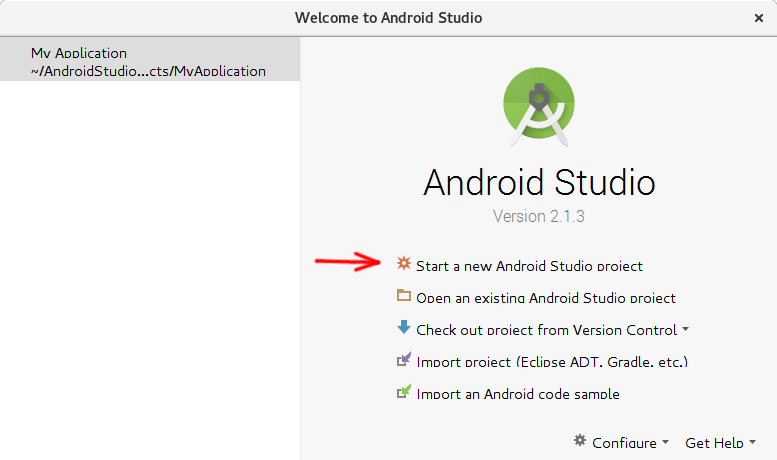
\includegraphics[scale=0.3]{chapters/ch02/images/1_welcome_screen}
\end{center}

The left side panel lists the projects that you've already created. The right side panel contains a bunch of buttons and options. You can import projects or open legacy code through here. At the bottom of this window, there is a configure button with a ``cog'' icon. Clicking it brings a drop down menu from where you can install or update various features and plugins. For now we will skip it.

From the right side panel, click on ``Start a new Android Studio project'' option (marked by the red arrow). This will take you to the configuration screen shown below:

\begin{center}
	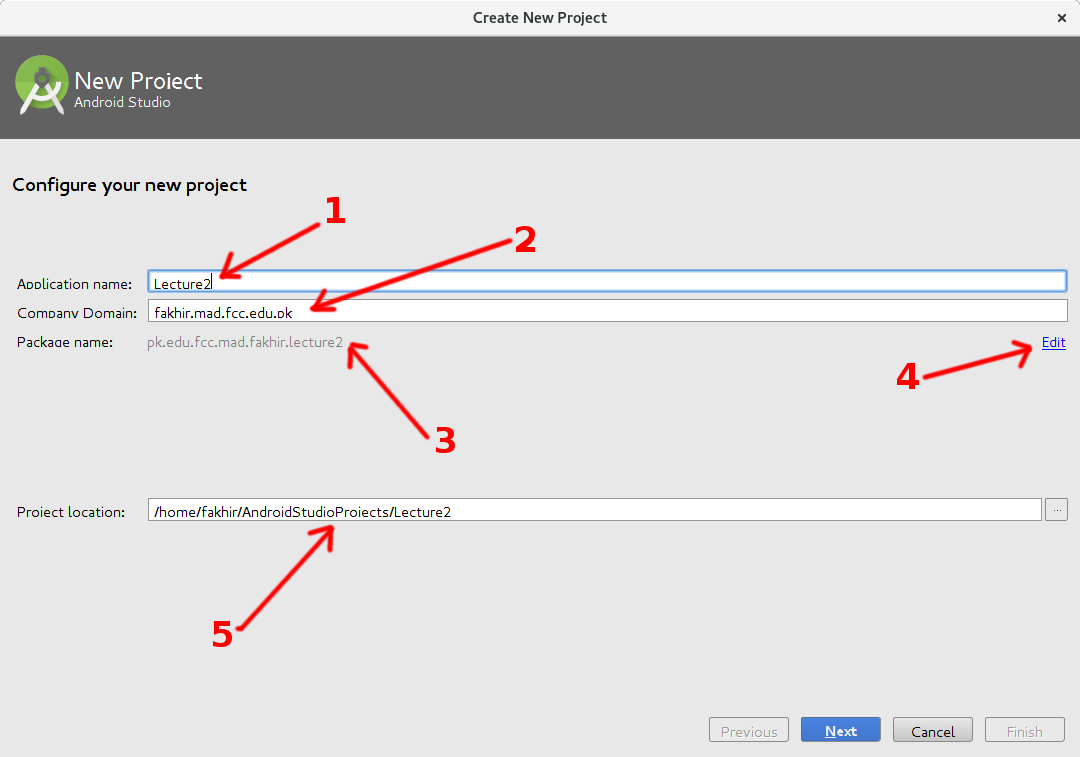
\includegraphics[scale=0.3]{chapters/ch02/images/2_app_name}
\end{center}

Each of the numbered arrows are explained in the list below:

\begin{enumerate}
	\item \textit{Application name:} This is the name of your application. You can change it to anything you like. For this exercise let's rename it to ``Lecture 2''.
	\item \textit{Company Domain:} This is a global identifier that will uniquely identify you app. This has to be different from all of the apps currently available on the android app store (or google play store). You can put it any valid string as long as it is unique.
	\item \textit{Package name:} Android studio automatically generates a string according to the previously entered information. You might've seen similar structure when programming for Java language.
	\item \textit{Edit:} If you need to give your own package name, then just click on ``Edit'' at the right side. We will leave the default value for now.
	\item \textit{Project location:} The complete path of the current project. You can change it if you like, but again we will leave the default value.
\end{enumerate}

Click next to go to the ``Target Android Devices'' screen. That'll bring you to the following window:

\begin{center}
	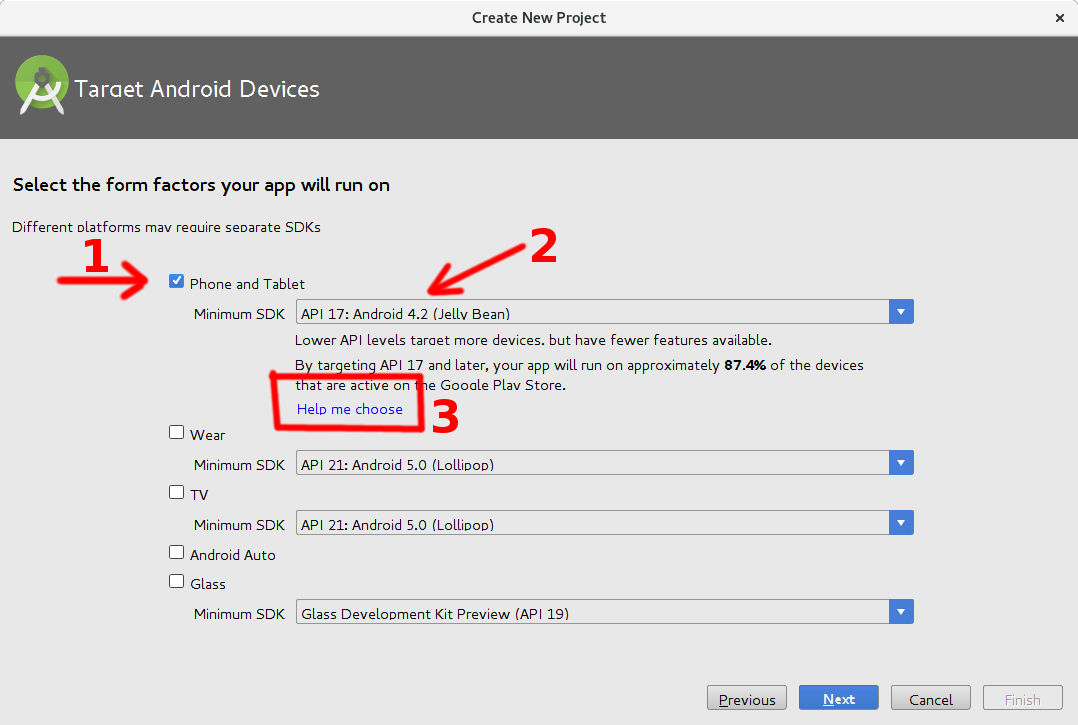
\includegraphics[scale=0.2]{chapters/ch02/images/3_os_select}
\end{center}

\begin{enumerate}
	\item In this course we will be developing only for phones and tables. Check this option and ignore the others.
	\item \textit{Minimum SDK:} This is the minimum version of android API that your app will run on. For example if you selected API 21 (Lolipop) as minimum API then your app will not run on any mobile device that has android version 19 (Kitkat) or less installed on it. For now select API 17 so that our app runs on approximately 87.4\% of the devices out there. 
	\item If you want to see the complete compatibility chart, click ``Help me choose''. This will show you approximate number of devices your app will run on.
\end{enumerate}

Hit next button to go to the ``Add an Activity to Mobile'' screen:

\begin{center}
	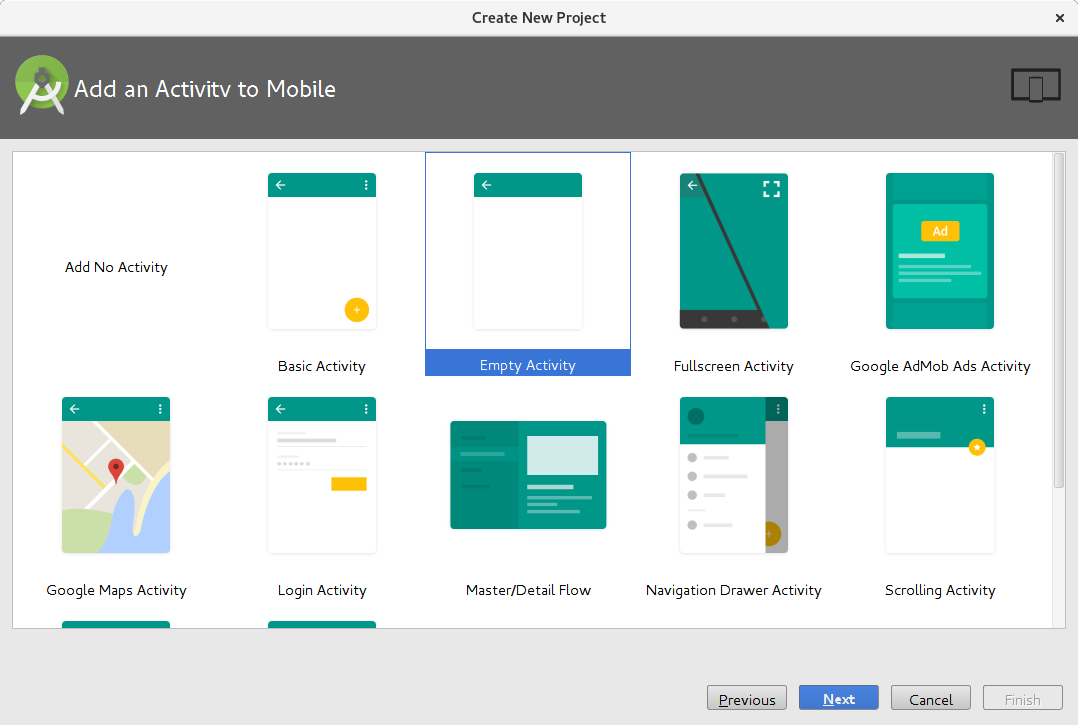
\includegraphics[scale=0.2]{chapters/ch02/images/4_activity}
\end{center}

Select ``Empty Activity'' and hit next to go to ``Customize the Activity'' screen. Leave the default options as is and click finish to create the project.

\section{Tour of Android Studio IDE}
Once your project is successfully created, you will see the following screen with some files already opened up:

\begin{center}
	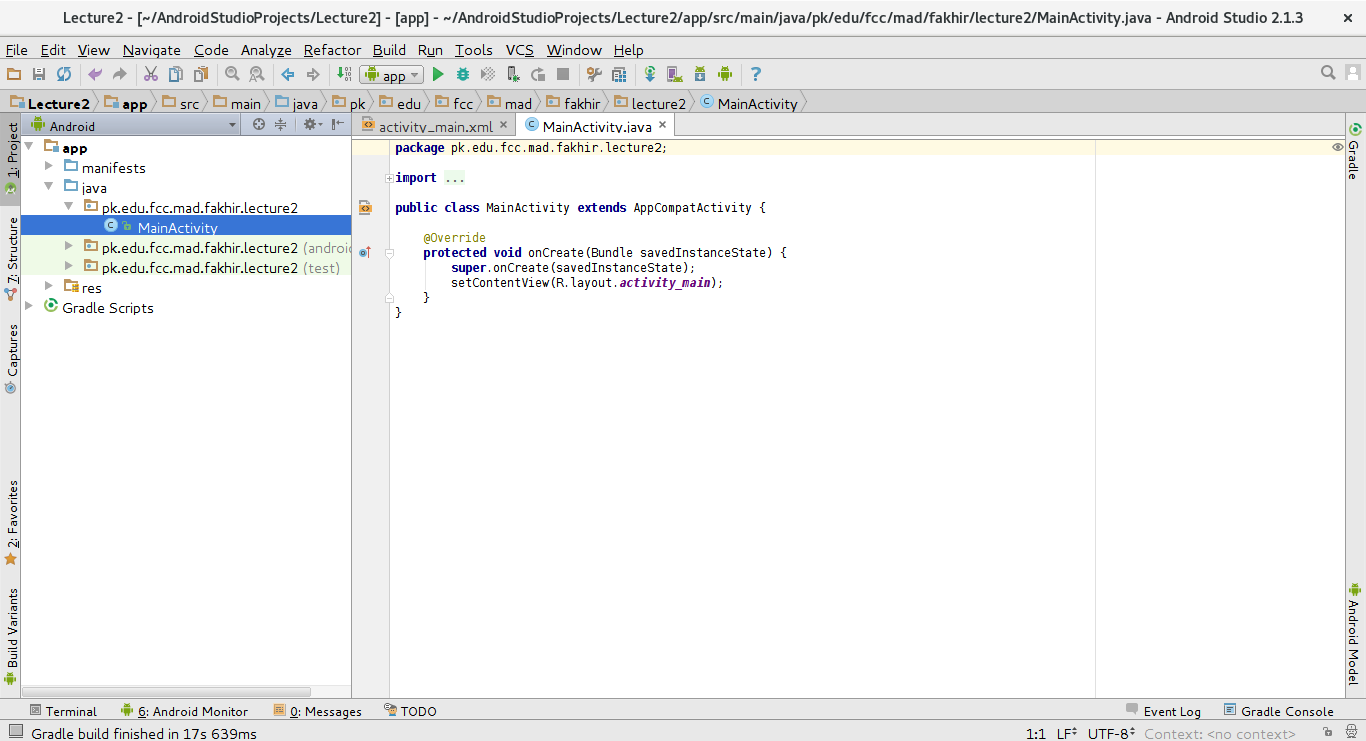
\includegraphics[scale=0.2]{chapters/ch02/images/5_android_studio}
\end{center}

The left side panel shows the project structure. This panel basically shows the assets, code, configuration files related to this project:

\begin{center}
	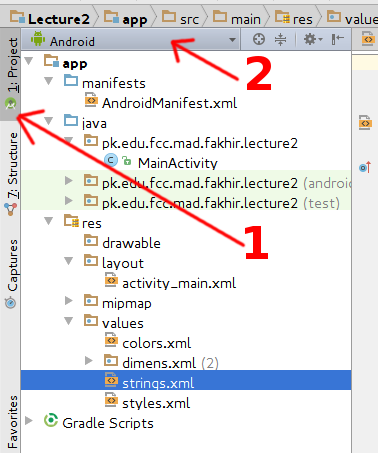
\includegraphics[scale=0.3]{chapters/ch02/images/6_project_panel}
\end{center}

\begin{enumerate}
	\item Make sure that the ``Project'' tab is selected. This will show the overall bird's eye view of the current project. You can view the project structure in various ways as mentioned below.
	\item Now if ``Android'' is selected, this will show you the ``Logical'' layout. Android studio will group and show similar items under the same label even if these items are actually placed in different directories.
	\item If you select ``Project'' instead of ``Android'', this will show you the actual physical structure of the project including all the actual sub-directories. Both the views are useful but for now we will be using ``Project $\rightarrow$ Android''.
	\item ``Structure'' tab shows the code structure of the project i.e: Class hierarchies, member functions, member variables etc.
\end{enumerate}

In the middle of the screen this area is the editor panel. Here we write and modify code. Two files are already opened, one java and other XML. We will look into detail what these files exactly do. Click on the ``activity\_main.xml'' tab to bring ot the layout.

\begin{center}
	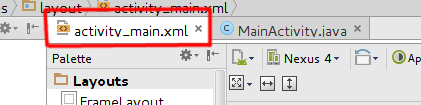
\includegraphics[scale=0.4]{chapters/ch02/images/7_editor}
\end{center}

Clicking any layout XML file opens up the design mode. Notice how the editor area is now converted into a number of panels housing lot of different options:

\begin{center}
	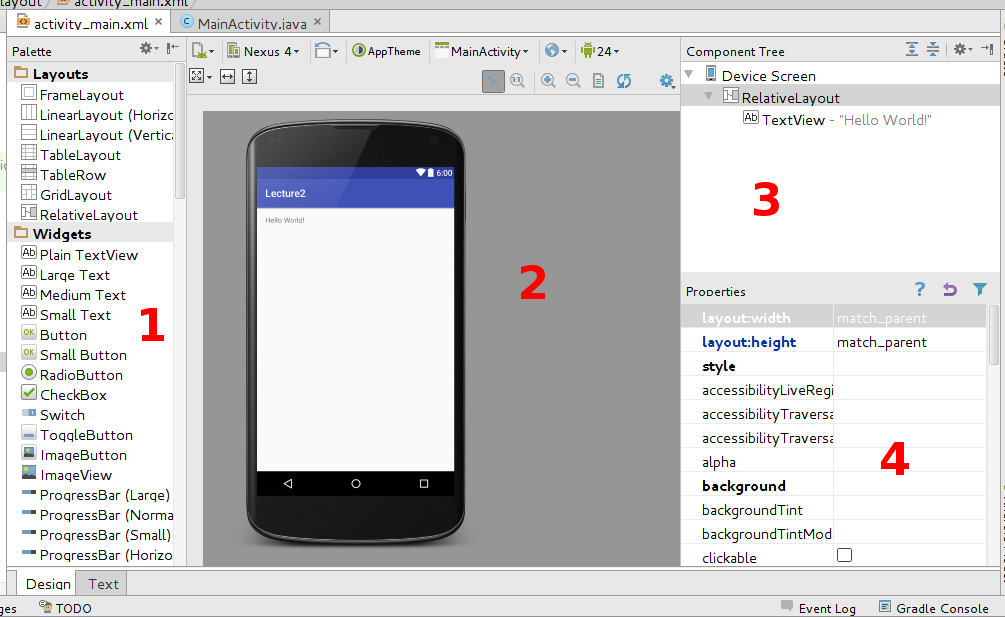
\includegraphics[scale=0.3]{chapters/ch02/images/8_design}
\end{center}

\begin{enumerate}
	\item The panel at the left is referred to as the ``Palette panel''. This panel contains all of the layouts, buttons, widgets, gadgets that you can use to make very complex user interfaces. Just drag anything from here and drop it onto the mobile preview area.
	\item This is the mobile preview area. This shows how your layout will look on the actual device!!! (You don't even have to run your app on the emulator or physical device). 
	
	\textbf{IMPORTANT NOTE: This ONLY previews the layout. This will NOT run your java code. To run your logic code you must run your app on an emulator or a dvice.}
	\item The panel on the top right is called ``Component tree'' panel. This shows hierarchical relationship between different components and controls (for example a button can contain a label inside it etc). 
	\item The panel on lower right shows all of the possible properties of the currently selected component. Here you can change size, color, font, physical outlook etc of any control that you can imagine.
\end{enumerate}

Let's explore the preview area a little bit more. 

\begin{center}
	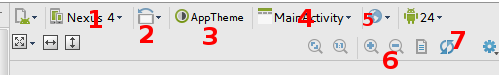
\includegraphics[scale=0.6]{chapters/ch02/images/9_design_area}
\end{center}

\begin{enumerate}
	\item You can preview your layout on any android device (phone, tablet, watch or even TV). Clicking on this button will bring down a drop-down menu having a lot of options. You can choose any of the devices to test your layouts onto.
	\item You can test your layout (or user interface in other words) on different orientations. Click this button to switch between portrait and landscape modes.
	\item You can also change the overall theme of your app but for now we will not be covering this.
	\item You can make multiple layouts or screens in your app and you can individually test any of these. Since we have only one layout for our app, the drop-down menu shows only one!
	\item You can also change the language of your app for example from english to arabic.
	\item This zooms and unzooms the preview area.
	\item Refreshes the preview area to update latest changes.
\end{enumerate}

The layouts are actually XML files containing source code. Android studio reads that code and draws the layout in design view. In order to view the actual XML source code, click the ``Text'' tab on bottom left side of the design area, right underneath the ``Palette panel'':

\begin{center}
	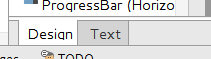
\includegraphics[scale=0.6]{chapters/ch02/images/10_textMode}
\end{center}

This will transform the entire middle area from drag/drop design mode to a source code editor:

\begin{center}
	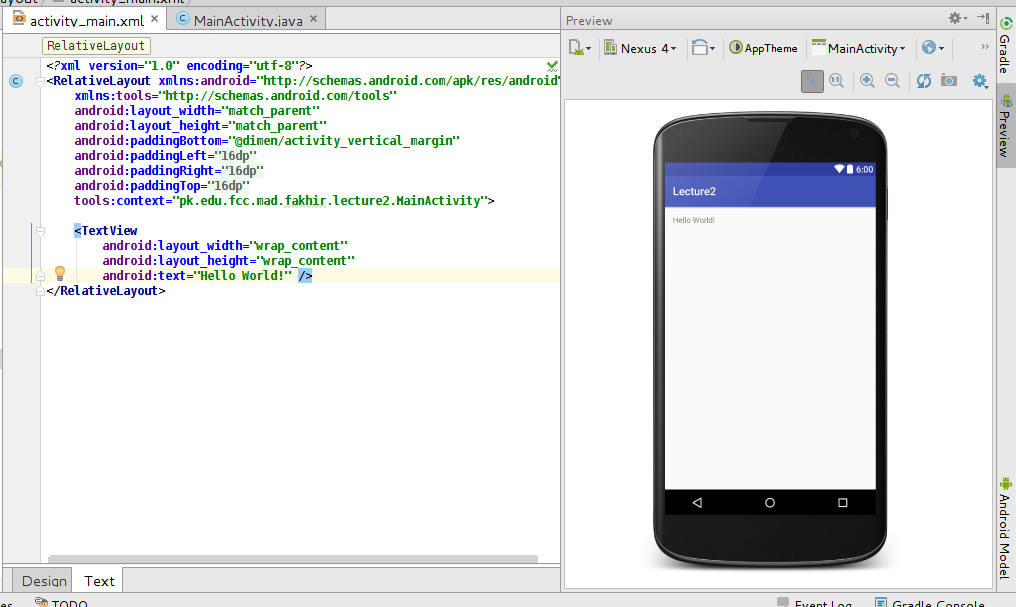
\includegraphics[scale=0.3]{chapters/ch02/images/11_textMode}
\end{center}

On the left side you can see the complete XML source code for the layout. On the right side you can see the preview window. If you like you can make very complex layouts right in this XML text mode!

\section{Important concepts}
Let's pause for a moment and let's take a look at some important concepts.

\subsection{Activity}
\label{TOAS:activity}
An \textbf{Activity} can be thought of as a screen. Like a university website can have multiple pages, about, home, faculty, students etc. Each website has a different ``layout'' or ``appearance''. Similarly a mobile app can have multiple screens or activities.

Each activity is made up of two components: 
\begin{itemize}
	\item Exactly ONE Java file (the brains / logic)
	\item At least ONE XML file (the beauty)
\end{itemize}

\begin{center}
	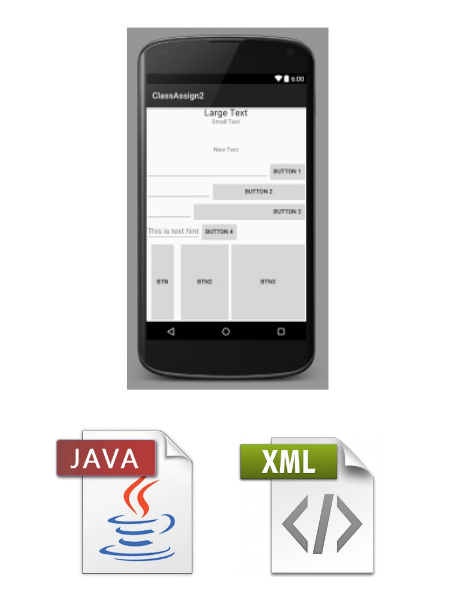
\includegraphics[scale=0.4]{chapters/ch02/images/12_activity}
\end{center}


Our app has got only one activity named \texttt{\textbf{Main}} having ``\texttt{MainActivity.java}'' and ``\texttt{activity\_main.xml}'' attached to it. We can create as many activities as we want within an app, as we will see later down the road.

\subsection{View}
You can think of the views simply as ``(invisible) interactive rectangles''. Pretty much everything is a view. A button is a view, edit box is a view, label is a view etc. There can even be invisible views. Special views that can contain other views within them are called ``View Groups''. Views \textbf{can not} contain any other views. But view groups \textbf{can} contain other views or even view groups. View groups are used to nicely format and align components on the screen.

\section{Simple layout}
Alright, enough theory, let's resume our app development. Open up ``activity\_main.xml'' if it is not already open and go to the design mode. Let's zoom it a bit. Click the zoom button a few times:

\begin{center}
	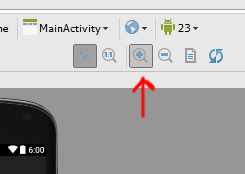
\includegraphics[scale=0.4]{chapters/ch02/images/14_zoom}
\end{center}

You will see \textbf{“Hello world”} written on the output screen. This is actually a UI control of type \texttt{TextView} placed on the screen. \texttt{TextView} displays text to the user and optionally allows them to edit it.

Go to the panel on the right, find the ``Component Tree'' view. The ``Component Tree'' shows all the UI controls, views, view groups placed onto the canvas in a hierarchical parent-child tree like structure. Select \texttt{TextView}. You can either directly select a control from the canvas or the from ``Component Tree'':

\begin{center}
	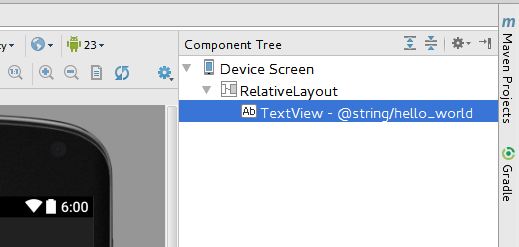
\includegraphics[scale=0.4]{chapters/ch02/images/15_component_tree}
\end{center}

Let's modify some properties of the text view. Under the ``Component Tree'' you will see the properties panel. It lists all of the properties of a selected widget. This panel is ``context sensitive''. It means that the values listed will change depending on the type of widget currently selected. Since we've already selected \texttt{TextView}, find \texttt{textSize} and change it to \textbf{60dp}. The `dp' means device independent points, these are not raw pixels. Also set the \texttt{textStyle} to `Bold' and `Italic':

\begin{center}
	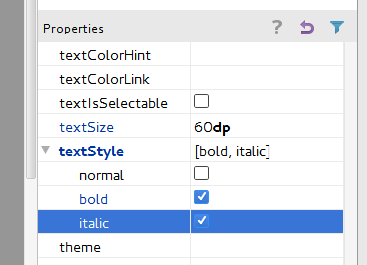
\includegraphics[scale=0.4]{chapters/ch02/images/16_bold_italic}
\end{center}

There are two ways to specify the color. Simplest is the \#RGB. This is means that only 16 levels for each of the red, green and blue colors, a total of only 4096 color combinations. Second way is to specify the entire \#RRGGBB format. This one is 256 levels for each red, green,blue; a total of 16 million color combinations.

While \texttt{TextView} is still selected, enter \#002 in the background field:

\begin{center}
	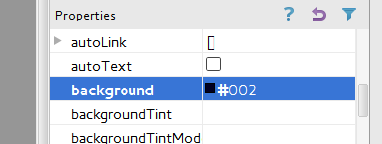
\includegraphics[scale=0.4]{chapters/ch02/images/17_background}
\end{center}

Enter \#ffff33 in \texttt{textColor}:

\begin{center}
	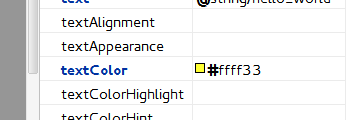
\includegraphics[scale=0.4]{chapters/ch02/images/18_text_color}
\end{center}

Select Nexus 10 tablet to see how our layout looks like on it:

\begin{center}
	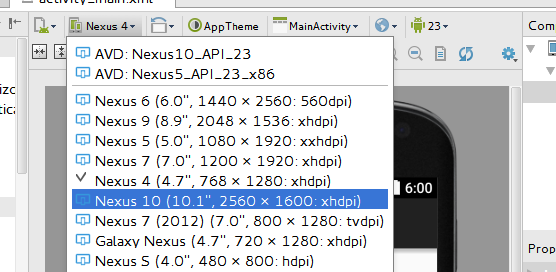
\includegraphics[scale=0.4]{chapters/ch02/images/19_nexus_10}
\end{center}

Now select Nexus 5:

\begin{center}
	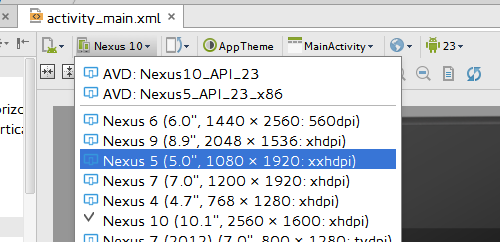
\includegraphics[scale=0.4]{chapters/ch02/images/20_nexus_5}
\end{center}

The mobile phone view may be a bit too zoomed in. Click on `Zoom to fit' button:

\begin{center}
	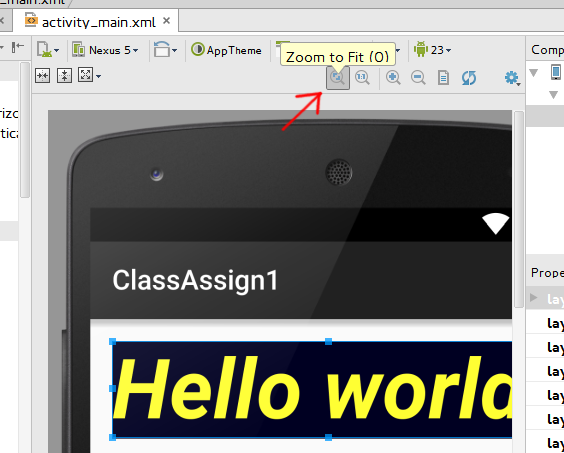
\includegraphics[scale=0.4]{chapters/ch02/images/21_zoom}
\end{center}

To see how your layout looks like on a different orientation such as landscape mode, click the change orientation button:

\begin{center}
	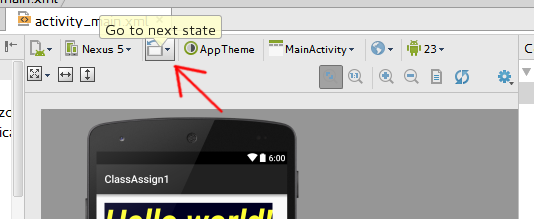
\includegraphics[scale=0.4]{chapters/ch02/images/22_state}
\end{center}

Finally click the green play button to run the app on device or the emulator:

\begin{center}
	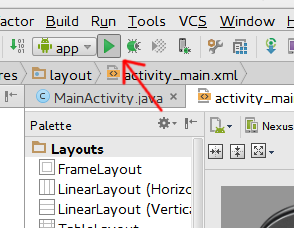
\includegraphics[scale=0.4]{chapters/ch02/images/23_play}
\end{center}

You should see the following on your mobile or the emulator. Quick tip about emulator: To change its orientation from portrait to landscape and vice versa just press `ctrl+F12':

\begin{center}
	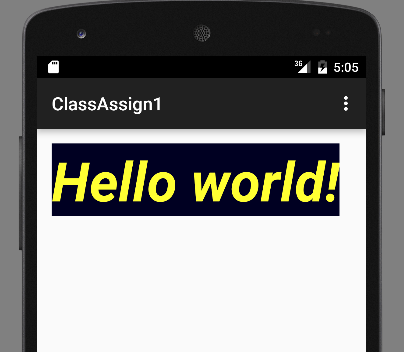
\includegraphics[scale=0.4]{chapters/ch02/images/24_device}
\end{center}

\section{Exercise}
Try to make an interface shown in the following diagram. If you don't understand anything then don't worry we will cover it in detail in the upcoming classes.

\begin{center}
	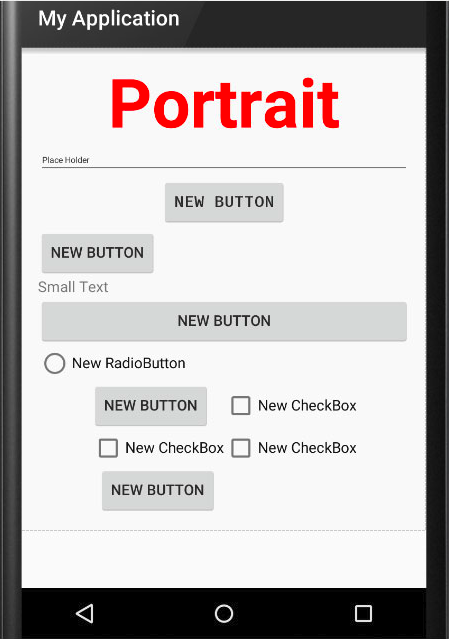
\includegraphics[scale=0.4]{chapters/ch02/images/25_activity1}
\end{center}